\input{./content_Praesentation/Packete_und_Deklarationen}
%!Tex Root = ../Main.tex
% ./content/Packete_und_Deklarationen.tex
% ./content/Einführung.tex
% ./content/Implementierung.tex
% ./content/Implementierung2.tex
% ./content/Implementierung3.tex
% ./content/Vorführung.tex
% ./content/Qualitätssicherung.tex
% ./content/Appendix.tex

\newtcbinputlisting{\codebox}[2][]{
  listing file={#2},
  enhanced, colframe=PrimaryColor,colback=BoxColor, fonttitle=\small, arc=1mm, bottom=1mm, top=1mm, left=1mm, right=1mm, #1, listing only, listing engine=minted, minted style=colorful, halign title=center, drop fuzzy shadow,
}

% minted options={fontsize=\tiny,linenos=false,breaklines,breakafter={_}, breakbefore={(}, breakaftersymbolpre={}, breakaftersymbolpost={}, breakbeforesymbolpre={}, breakbeforesymbolpost={}, breaksymbolsepleft=2mm, breaksymbolsepright=0mm, breakindent=0mm, breaksymbolindentleft=5mm, breaksymbolindentright=0mm, numbersep=0mm, escapeinside=||}

\newtcblisting{terminal}{
enhanced, colframe=SecondaryColor, colback=BoxColor, hbox, fonttitle=\small, arc=1mm, bottom=1mm, top=1mm, left=1mm, right=1mm, listing only, listing engine=minted, halign title=center, drop fuzzy shadow, minted language=text, minted options={fontsize=\tiny,linenos=false,autogobble,breaklines,breakafter={_}, breakbefore={(}, breakaftersymbolpre={}, breakaftersymbolpost={}, breakbeforesymbolpre={}, breakbeforesymbolpost={}, breaksymbolsepleft=2mm, breaksymbolsepright=0mm, breakindent=0mm, breaksymbolindentleft=5mm, breaksymbolindentright=0mm, numbersep=0mm, escapeinside=||}
}
\newtcolorbox{Code_Frame}[2][]{enhanced, drop fuzzy shadow, arc=1mm, bottom=1mm, top=0mm, left=1mm, right=1mm, boxrule=1mm, halign title=center, fonttitle=\tiny, interior style={fill=white}, frame style={color=PrimaryColor}, title={#2}, #1}
% , sharpish corners

% \newtcbinputlisting{codeframe}[2][]{
%   listing file={#2},
%   enhanced, colframe=PrimaryColor,colback=BoxColor, fonttitle=\tiny, arc=1mm, bottom=1mm, top=1mm, left=1mm, right=1mm, #1, listing only, listing engine=minted, minted style=colorful, halign title=center, drop fuzzy shadow,
% }

\DeclareTCBInputListing{\codeframe}{ s o m }{listing file={#3},
enhanced,colback=BoxColor,IfBooleanTF={#1}{colframe=SecondaryColor}{colframe=PrimaryColor},fonttitle=\tiny,arc=1mm,bottom=1mm,top=1mm,left=1mm,right=1mm,#2,listing only,listing engine=minted,minted style=colorful,halign title=center,drop fuzzy shadow}

\newtcolorbox{File}[1][]{enhanced, hbox, drop fuzzy shadow, arc=1mm, bottom=1mm, top=1mm, left=1mm, right=1mm, notitle, interior style={fill=PrimaryColor}, frame empty, halign=center, fontupper=\color{white}\tiny, #1}

\newtcbinputlisting{\numberedcodebox}[2][]{
listing file={#2},
enhanced, colframe=PrimaryColor,colback=BoxColor, fonttitle=\small, arc=1mm, #1, listing only, listing engine=minted, minted style=colorful, halign title=center, drop fuzzy shadow, overlay={\begin{tcbclipinterior}\fill[PrimaryColor] (frame.south west) rectangle ([xshift=4mm]frame.north west);\end{tcbclipinterior}}
}
% minted options={fontsize=\tiny,breaklines,autogobble,linenos,numbersep=3mm, highlightcolor=SecondaryColor,escapeinside=||}

\DeclareTotalTCBox{\inlinebox}{ s v }
{verbatim,colback=SecondaryColorDimmed,colframe=SecondaryColor}
{\IfBooleanTF{#1}%
{\textcolor{SecondaryColor}{\setBold >\enspace\ignorespaces}#2}%
{#2}}

\DeclareTotalTCBox{\key}{ m }
{verbatim,colback=SecondaryColorDimmed,colframe=SecondaryColor}
{$\mathtt{#1}$}


\title{Titel der Präsentation}
\subtitle{Untertitel der Präsentation}
\author{Autor der Präsentation}
\institute{Institut dem die Präsentation zuzuordnen ist}
\date{\today}
% \logo{\includegraphics[height=0.5cm]{./figures/logo.png}}

\includeonly{
  ./content_Praesentation/Kapitel1,
  ./content_Praesentation/Kapitel2,
}

\def\hide{0}

\begin{document}

\begin{withoutheadline}
  \begin{withoutfootline}
    \begin{frame}
      \titlepagesecond
    \end{frame}
  \end{withoutfootline}

  \begin{frame}{Gliederung}
    \tableofcontents[hideallsubsections]
  \end{frame}
\end{withoutheadline}

%!Tex Root = ../Vorlage_Praesentation.tex
% ./Packete.tex
% ./Design.tex
% ./Deklarationen.tex
% ./Kapitel2.tex

\if\hide0\section{Kapitel 1}\fi

\begin{frame}[label={kapitel1}]{Kapitel 2}{Beispiel Definitionsbox}
  \begin{block}{Test \notebook}
    \lipsum[1]
  \end{block}
\end{frame}

\begin{frame}{Kapitel 1}{Beispiel für Tabelle}
  \scriptsize
  \begin{table}[H]
    \center
    \begin{NiceTabular}{X[1,c]X[2,l]}[rules/color=PrimaryColor] % {\linewidth}{|C|C|L|L|}
      \CodeBefore
      \chessboardcolors{white}{BoxColor}
      \rowcolor{PrimaryColor}{1}
      \Body
      \textcolor{white}{Spalte 1} & \textcolor{white}{Spalte 2} \\
      \scripttt{row1} & \alert{Beschreibung} für \scripttt{row1}. \\
      \scripttt{row2} & \aalert{Beschreibung} für \scripttt{row2}. \\
      \bottomrule
    \end{NiceTabular}
    \caption{Beispiel.}
  \end{table}
\end{frame}

\begin{frame}{Kapitel 2}{Beispiel für Diagram}
  \begin{figure}
    \begin{transformation}[0.2][0.2][0.5]
      {\dq}{4}\enspace {*}\enspace {2}{\dq}
      \arrowxx{Aktion 1}{Aktion 2}
      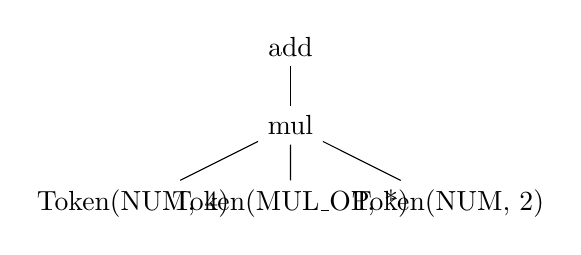
\begin{tikzpicture}[auto, align=center, sibling distance=2cm, level distance=1cm, baseline=(current  bounding  box.center)]
        \node {\tinytt{add}}
        child {node {\tinytt{mul}}
          child {node {\tinytt{Token(NUM, \dq 4\dq)}}}
          child {node {\tinytt{Token(MUL\_OP, \dq *\dq)}}}
          child {node {\tinytt{Token(NUM, \dq 2\dq)}}}};
      \end{tikzpicture}
    \end{transformation}
    \caption{Untertitel.}
  \end{figure}
\end{frame}

\begin{frame}{Kapitel 2}{Weiteres Beispiel für Diagram}
  \begin{equation}
    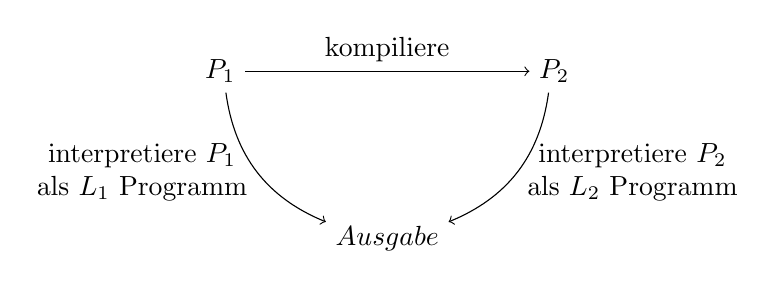
\begin{tikzpicture}[auto, baseline=(current  bounding  box.center)]
      \node (program1) at (135:3) {$P_{1}$};
      \node (program2) at (45:3) {$P_{2}$};
      \node (output)  at (270:0) {$Ausgabe$};

      % https://tex.stackexchange.com/questions/24372/how-to-add-newline-within-node-using-tikz
      \draw[->] (program1) to node[above] {kompiliere} (program2);
      \draw[->] (program1) to[bend right] node[left, align=center] {interpretiere $P_{1}$\\ als $L_{1}$ Programm} (output);
      \draw[->] (program2) to[bend left] node[right, align=center] {interpretiere $P_{2}$\\ als $L_{2}$ Programm} (output);
    \end{tikzpicture}
  \end{equation}
\end{frame}

%!Tex Root = ../Vorlage_Praesentation.tex
% ./Packete.tex
% ./Design.tex
% ./Deklarationen.tex
% ./Kapitel1.tex

\if\hide0\section{Kapitel 2}\fi

\begin{frame}[fragile]{Kapitel 1}{Beispiele für Codeboxen}
  \begin{columns}
    \begin{column}{0.4\textwidth}
      \codebox[title=Codebeispiel, remember as=codebeispiel1, minted language=c, minted options={highlightlines={1,3-7}}]{./code_examples/example.c}
    \end{column}
    \hfill
    \begin{column}{0.4\textwidth}
      \begin{linenums}
        \numberedcodebox[remember as=codebeispiel2, minted language=c, minted options={}]{./code_examples/example.c}
      \end{linenums}
    \end{column}
  \end{columns}
  \begin{tikzpicture}[overlay,remember picture,line width=1mm,draw=PrimaryColor, font=\small, draw=SecondaryColor]
    \draw[->] (codebeispiel1.east) to[bend left] node[above, align=center] {Mehrzeiliger\\ Text} (codebeispiel2.west);
  \end{tikzpicture}
\end{frame}

\begin{frame}[fragile, label={kapitel2}]{Kapitel 2}{Beispiele für Inline Boxen}
    \begin{itemize}
      \coloritem \inlinebox{arg} aus \inlinebox*{command arg}.
      \coloritem \key{\Uparrow-Tab}.
    \end{itemize}
\end{frame}

\begin{frame}{Kapitel 2}{Beispiel für hierarchisch aufgebaute Codebeispiele}
  \centering
  \begin{file}[remember as=input]
    Start
  \end{file}
  \vspace{0.1cm}
  \begin{codeframe}*[remember as=frameone]{Frame 1}
    \codebox[title=Codebeispiel 1, width=0.4\linewidth, nobeforeafter, minted language=text, equal height group=A, minted options={highlightlines={2}}]{./code_examples/example2.special}
    \hfill
    \codebox*[title=Codebeispiel 2, width=0.4\linewidth, nobeforeafter, minted language=text, equal height group=A, minted options={highlightlines={3}}]{./code_examples/example2.special}
  \end{codeframe}
  \vspace{0.1cm}
  \begin{file}[remember as=conta]
    ...
  \end{file}
  \begin{tikzpicture}[overlay,remember picture,line width=1mm,draw=PrimaryColor, font=\tiny]
    \draw[->, color=SecondaryColor] (input.south) to node[right=0.25cm, align=center] {\textcolor{black}{Verbindung 1}} (frameone.north);
    \draw[->] (frameone.south) to node[right=0.25cm, align=center] {Verbindung 2} (conta.north);
  \end{tikzpicture}
\end{frame}

\begin{frame}[fragile]{Kapitel 2}{Beispiel für Terminal}
  \centering
  \begin{terminal}
    |\prompt| command arg
    |\customprompt| command arg
  \end{terminal}
  %   % |\prompt|
\end{frame}


\section{Literatur}

\begin{frame}{Bücher}
  \printbibliography[type=book,heading=subbibliography,title={Bücher}]
\end{frame}

\begin{frame}{Artikel}
  \printbibliography[type=article,heading=subbibliography,title={Artikel}]
\end{frame}

\begin{frame}{Vorlesungen}
  \printbibliography[type=unpublished,heading=subbibliography,title={Vorlesungen}]
\end{frame}

\begin{frame}{Online}
  \printbibliography[type=online,heading=subbibliography,title={Online}]
\end{frame}

\begin{frame}{Sonstige}
  \printbibliography[nottype=book, nottype=article, nottype=online, nottype=unpublished,heading=subbibliography,keyword=wikikeyword,title={Sonstige Quellen}]
\end{frame}
\end{document}
